\documentclass[11pt]{article}
\usepackage[margin=1in]{geometry}
\usepackage[T1]{fontenc}
\usepackage[utf8]{inputenc}
\usepackage{lmodern}
\usepackage{amsmath,amssymb,amsthm}
\usepackage{booktabs,tabularx,multirow}
\usepackage{graphicx}
\usepackage{microtype}
\usepackage{xcolor}
\usepackage[numbers,sort&compress]{natbib}
\usepackage{algorithm}
\usepackage[noend]{algpseudocode}
\usepackage{caption}
\usepackage{enumitem}
\usepackage{tikz}
\usetikzlibrary{positioning,arrows.meta,fit,backgrounds}
\usepackage[colorlinks=true,linkcolor=blue!50!black,citecolor=blue!50!black,urlcolor=blue!50!black]{hyperref}
\usepackage[capitalise,noabbrev]{cleveref}

\newtheorem{proposition}{Proposition}
\newtheorem{corollary}{Corollary}
\newtheorem{lemma}{Lemma}
\theoremstyle{remark}
\newtheorem{remark}{Remark}
\captionsetup{font=small,labelfont=bf}
\setlength{\tabcolsep}{4pt}
\setlist{nosep,leftmargin=*}

% generated by build_assets.py -- do not edit
\newcommand{\rThreeAll}{0.812}
\newcommand{\rThreeLo}{0.752}
\newcommand{\rThreeHi}{0.866}
\newcommand{\rThreeSarimax}{0.810}
\newcommand{\pairSar}{1.002}
\newcommand{\pairSarLo}{0.966}
\newcommand{\pairSarHi}{1.041}
\newcommand{\pairSarWins}{27}
\newcommand{\pairNl}{0.812}
\newcommand{\pairNlLo}{0.752}
\newcommand{\pairNlHi}{0.866}
\newcommand{\pairNlWins}{52}
\newcommand{\pairDl}{0.804}
\newcommand{\pairDlLo}{0.765}
\newcommand{\pairDlHi}{0.844}
\newcommand{\pairDlWins}{56}
\newcommand{\pairFits}{0.652}
\newcommand{\pairFitsLo}{0.609}
\newcommand{\pairFitsHi}{0.702}
\newcommand{\pairFitsWins}{59}
\newcommand{\pairStsf}{0.277}
\newcommand{\pairStsfLo}{0.234}
\newcommand{\pairStsfHi}{0.323}
\newcommand{\pairStsfWins}{60}
\newcommand{\pairArx}{0.582}
\newcommand{\pairArxLo}{0.378}
\newcommand{\pairArxHi}{0.797}
\newcommand{\pairArxWins}{30}
\newcommand{\pairChr}{1.250}
\newcommand{\pairChrLo}{1.178}
\newcommand{\pairChrHi}{1.337}
\newcommand{\pairChrWins}{9}
\newcommand{\pairTtmZ}{0.747}
\newcommand{\pairTtmZLo}{0.704}
\newcommand{\pairTtmZHi}{0.795}
\newcommand{\pairTtmZWins}{57}
\newcommand{\pairTtmF}{0.771}
\newcommand{\pairTtmFLo}{0.699}
\newcommand{\pairTtmFHi}{0.844}
\newcommand{\pairTtmFWins}{50}
\newcommand{\kLebThousand}{0.811}
\newcommand{\kChrThousand}{0.649}
\newcommand{\kChrBdg}{0.539}
\newcommand{\kLebBdg}{0.787}
\newcommand{\fpMean}{415}
\newcommand{\fpMax}{1{,}020}
\newcommand{\fpOverMean}{3.7}
\newcommand{\fpOverMax}{2.0}
\newcommand{\covThree}{0.904}
\newcommand{\ttmZsFlops}{15.6}
\newcommand{\ttmFtFlops}{55.6}
\newcommand{\rTwoAll}{0.767}
\newcommand{\rTwoLo}{0.657}
\newcommand{\rTwoHi}{0.858}
\newcommand{\rTwoSar}{0.999}
\newcommand{\rTwoChr}{1.161}
\newcommand{\rTwoFrozen}{1.107}
\newcommand{\rTwoFrozenRatio}{0.693}
\newcommand{\rTwoFrozenCat}{2}
\newcommand{\rOneAll}{5.20}
\newcommand{\instrMin}{3.2}
\newcommand{\instrMax}{6.0}
\newcommand{\usMin}{31}
\newcommand{\usMax}{57}
\newcommand{\stateKB}{73}
\newcommand{\peakMin}{37}
\newcommand{\peakMax}{48}
\newcommand{\cpiA}{1.62}
\newcommand{\cpiB}{1.57}
\newcommand{\eqDevF}{28}
\newcommand{\eqDevD}{29}
\newcommand{\eqThree}{54}
\newcommand{\misAccA}{10}
\newcommand{\misOrcMedA}{18.2}
\newcommand{\misOrcMaxA}{33.4}
\newcommand{\misAccB}{0}
\newcommand{\misOrcMedB}{0.7}
\newcommand{\misOrcMaxB}{5.2}
\newcommand{\misAccC}{0}
\newcommand{\misOrcMedC}{0.0}
\newcommand{\misOrcMaxC}{0.2}
\newcommand{\misThr}{5.63}
\newcommand{\simRuns}{700}
\newcommand{\simNullRuns}{400}
\newcommand{\simNullFalse}{0}
\newcommand{\simPTwoFdr}{0.090}
\newcommand{\simPThreeFdr}{0.077}
\newcommand{\simPTwoRuns}{7}
\newcommand{\simPThreeRuns}{10}
\newcommand{\simPTwoPool}{0.045}
\newcommand{\simPThreePool}{0.038}
\newcommand{\simAffected}{17}
\newcommand{\simRemoved}{10}
\newcommand{\simFinal}{7}
\newcommand{\simPThreeFound}{2}
\newcommand{\ablRatio}{0.988}
\newcommand{\ablLo}{0.970}
\newcommand{\ablHi}{1.006}
\newcommand{\ablWins}{60}
\newcommand{\ablCost}{395}

\newcommand{\E}{\mathbb{E}}
\newcommand{\F}{\mathcal{F}}

\title{LEBRE: Online Forecasting with Evidence-Gated Structural Changes at a Cost of a Few Hundred Operations per Step}
\author{Silvano Lima\\[2pt]{\normalsize Independent researcher}\\{\normalsize\texttt{silvano.limadebarros@gmail.com}}\thanks{ORCID \href{https://orcid.org/0009-0000-3868-6747}{0009-0000-3868-6747}. Research record: \href{https://doi.org/10.5281/zenodo.23049103}{doi:10.5281/zenodo.23049103}.}}
\date{September 2026}

\begin{document}
\maketitle

\begin{abstract}
% generated by build_assets.py -- do not edit
We describe and evaluate LEBRE, an online one-step-ahead forecaster for a target driven by exogenous inputs, at a cost of a few hundred floating-point operations per step. The live model is a memory of the target's own past and an online linear regression on the current inputs, combined by dynamic model averaging. Structural changes (adding, removing or swapping a whole input, or refining its lag response) run in shadow and are accepted only when an anytime-valid e-process of predictive improvement crosses a level set by an online multiple-testing rule. The components are not new; the contribution is their integration at a nearly fixed cost, a condition under which predictive improvement may be read as structure, and a pre-registered evaluation. When the reference model is learned online, its estimation error is predictable, so a challenger can improve on it without new structure; the structural reading requires small reference misadjustment. In three sequential pre-registered evaluations on never-seen hydrology and building-energy series, the first (125 series) revealed an engineering failure. After the fix, on 40 and 60 series, LEBRE had the lowest error among the low-cost comparators evaluated (MSE relative to online NLinear 0.812 on 60 series, 95\% CI 0.752--0.866) and no catastrophic series; it tied a per-series SARIMAX with inputs and had about 25\% higher error than Chronos-2 with covariates. The pre-declared cost contract was narrowly missed (+3.7\% mean, +2.0\% peak). A C99 port ran on a simulated Cortex-M4F at 3.2--6.0 thousand instructions per step with 73 KB of state. The testing mechanism did not improve accuracy over switching all inputs on. Code, pre-registrations and per-series result tables are public.

\end{abstract}

\section{Introduction}

Many measurement systems need a forecast of the next value of a target on the device that measures it: the flow at a hydro plant, the load of a building, the output of a feeder. The target is driven by inputs that act with delay (rainfall, temperature, upstream flows). Such a forecaster must be cheap, must work without per-series tuning or offline training, and must not fail badly when the stream has gaps or changes. Foundation models for time series are accurate but cost $10^7$--$10^{10}$ operations per forecast \citep{ansari2025chronos2,ekambaram2024ttm}. Classical models with inputs, such as SARIMAX, need per-series maximum-likelihood fitting \citep{boxjenkins1970}. Very small neural forecasters exist \citep{lin2024sparsetsf,xu2024fits}, but they are usually univariate and batch-trained. Cheap online linear models, finally, do not know by themselves which inputs and delays matter.

LEBRE takes a specific point in this trade-off. It keeps a simple, cheap live model and treats every \emph{structural} change as an experiment. A challenger that differs from the live model by one change (a whole input, its lag response, or a latent residual state) runs in shadow. The change is accepted only when an anytime-valid e-process \citep{ramdas2023savi,grunwald2024safe} comparing the two forecasters \citep{choe2024comparing} crosses a level fixed by an online multiple-testing rule \citep{javanmard2018lond,xu2024elond}. The result is a forecaster whose structure (which inputs, which delays, since when, with how much evidence) is logged and can be audited.

\paragraph{Contributions.} We state them with their limits.
\begin{enumerate}
  \item \textbf{An integrated design} for a forecaster with inputs at a nearly fixed per-step cost. It combines whole-input units with hierarchical lag refinement, learned shadow challengers, tested removal and swap, and online multiple testing (\cref{sec:method}). The core mechanism is \emph{not} original: accepting structural changes by an e-process of predictive improvement with error control over a stream was proposed for online decision trees by \citet{amoukou2026trees}. Our contribution is the integration and extension to time series with inputs under a compute budget.
  \item \textbf{A condition of use} (\cref{sec:theory}). When the reference is learned online, the expected improvement of any predictable challenger is bounded by the reference's normalised estimation error, and that error is predictable from the past. A test of predictive improvement therefore compares \emph{methods}, not models \citep{giacomini2006}; it supports a structural reading only when the reference's misadjustment is small relative to the test margin. We verify this in simulation. The observation follows directly from known results, but we did not find it stated for this setting.
  \item \textbf{A pre-registered, sequential evaluation} on never-seen series (\cref{sec:protocol,sec:results}), including the failure found by the first evaluation and its confirmation on two later ones. It compares LEBRE with budget-class models, classical references and foundation models, and includes a false-change simulation and ablations.
  \item \textbf{An embedded feasibility check}: a C99 port that reproduces the reference implementation, measured on a simulated Cortex-M4F microcontroller.
\end{enumerate}
We do \emph{not} claim that LEBRE is the most accurate or the most economical forecaster. All statements are relative to the comparators, protocols and data described here.

\section{Related work}\label{sec:related}

\paragraph{Lightweight and foundation forecasters.} Linear and very small models are strong baselines for long-horizon forecasting: NLinear/DLinear \citep{zeng2023dlinear}, FITS \citep{xu2024fits} and SparseTSF \citep{lin2024sparsetsf}. They are typically univariate and batch-trained. Pre-trained foundation models range from about $10^6$ parameters (TTM, \citealp{ekambaram2024ttm}) to much larger ones that accept covariates (Chronos-2, \citealp{ansari2025chronos2}). On-device incremental learning with exogenous sensors has been demonstrated with small neural networks \citep{larapinal2026iot}, without statistical control of structure.

\paragraph{Anytime-valid comparison and online multiple testing.} E-processes give tests that remain valid under optional stopping \citep{ramdas2023savi,grunwald2024safe}. \citet{choe2024comparing} compare two sequential forecasters under a weak null of equal average score, building on the confidence sequences of \citet{howard2021cs}. LOND-type rules control the false discovery rate online \citep{javanmard2018lond}, including with e-values under arbitrary dependence \citep{xu2024elond}. Recent work treats hypotheses whose evidence keeps accumulating \citep{deheide2026closure} and doubly sequential settings \citep{yao2025sava}. \citet{choi2026corrections} accumulate evidence that a prespecified correction improves a predictive distribution. \citet{jha2026granger} test Granger non-causality sequentially with family-wise error control.

\paragraph{Structure selection.} \citet{amoukou2026trees} accept splits of online decision trees by an e-process on the prequential loss difference between incumbent and challenger, with family-wise control over the stream. This is the closest prior work to our mechanism. Recursive sparse identification of ARMAX systems offers asymptotic selection guarantees \citep{armax2025sparse}. Hierarchical testing \citep{meinshausen2008,yekutieli2008} motivates our parent-before-child refinement of lag bands.

\paragraph{Estimation error in predictive tests.} Tests of predictive ability compare forecasting methods, meaning a model together with its estimation procedure \citep{giacomini2006}. In nested batch comparisons, estimation error penalises the larger model \citep{clark2007}. \citet{han2026martingale} show that anytime-valid monitors can fire on real streams when the test's assumptions fail. \citet{fernandez2026promotion} report incumbent-induced biases in challenger promotion. Our \cref{sec:theory} makes the estimation-error issue explicit for e-processes that decide structure.

\section{Method}\label{sec:method}

\begin{figure}[t]
\centering
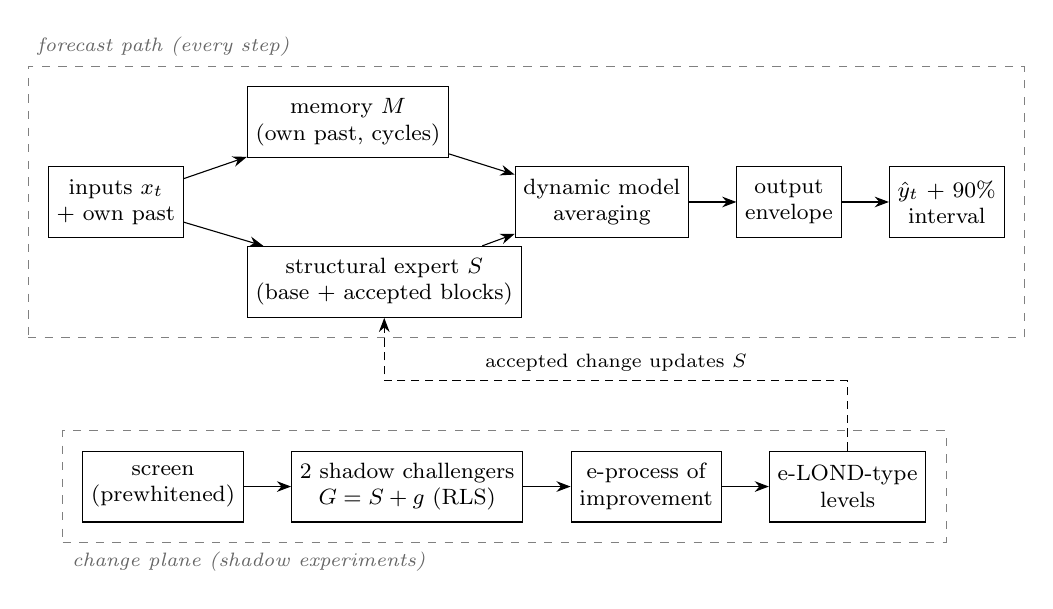
\begin{tikzpicture}[font=\footnotesize, node distance=4mm and 6mm,
  box/.style={draw, line width=0.4pt, align=center, minimum height=9mm, inner sep=3pt, fill=white},
  arr/.style={-{Stealth[length=1.8mm]}, line width=0.4pt},
  plane/.style={draw, dashed, line width=0.3pt, gray, inner sep=2.5mm},
  lbl/.style={font=\scriptsize\itshape, text=black!60}]
\node[box] (in) {inputs $x_t$\\+ own past};
\node[box, above right=1mm and 8mm of in] (M) {memory $M$\\(own past, cycles)};
\node[box, below right=1mm and 8mm of in] (S) {structural expert $S$\\(base + accepted blocks)};
\node[box, right=10mm of in, xshift=32mm] (C) {dynamic model\\averaging};
\node[box, right=of C] (O) {output\\envelope};
\node[box, right=of O] (Y) {$\hat y_t$ + 90\%\\interval};
\draw[arr] (in) -- (M); \draw[arr] (in) -- (S); \draw[arr] (M) -- (C); \draw[arr] (S) -- (C); \draw[arr] (C) -- (O); \draw[arr] (O) -- (Y);
\node[box, below=27mm of in, xshift=6mm] (sc) {screen\\(prewhitened)};
\node[box, right=of sc] (ch) {2 shadow challengers\\$G = S + g$ (RLS)};
\node[box, right=of ch] (ep) {e-process of\\improvement};
\node[box, right=of ep] (dec) {e-LOND-type\\levels};
\draw[arr] (sc) -- (ch); \draw[arr] (ch) -- (ep); \draw[arr] (ep) -- (dec);
\begin{scope}[on background layer]
\node[plane, fit=(in)(M)(S)(C)(O)(Y)] (fp) {};
\node[plane, fit=(sc)(ch)(ep)(dec)] (cp) {};
\end{scope}
\node[lbl, anchor=south west] at (fp.north west) {forecast path (every step)};
\node[lbl, anchor=north west] at (cp.south west) {change plane (shadow experiments)};
\draw[arr, densely dashed] (dec.north) |- node[pos=0.75, above, font=\scriptsize] {accepted change updates $S$} ([yshift=-8mm]S.south) -- (S.south);
\end{tikzpicture}
\caption{Architecture of LEBRE. The forecast path (top) runs at every step and is cheap. The change plane (bottom) proposes, tests and decides structural changes in shadow; only an accepted change alters $S$.}
\label{fig:arch}
\end{figure}

\cref{fig:arch} summarises the design and \cref{alg:step} gives one step. All constants are fixed across series (\cref{tab:params}); the environment only declares the sampling period(s).

\subsection{Live model}
\paragraph{Memory $M$.} A regression of the next increment on features of the target's own past, relative to the last value: reversion to a slow mean, last difference, seasonal naive and one-cycle increment, and a per-phase profile of increments. The features are inspired by the airline model and the Holt--Winters seasonal state \citep{boxjenkins1970,hyndman2008ets}. A second declared cycle (the week, for hourly building data) adds two features. Weights are learned by normalised LMS (NLMS) with step $0.05$ and scale-relative floors \citep{widrow1985,haykin2002}.
\paragraph{Structural expert $S$.} A linear regression on the current value of each standardised input and of the target's own past (the \emph{base}), plus the response blocks of accepted units, learned by NLMS with step $\mu=0.05$.
\paragraph{Combination.} Dynamic model averaging \citep{raftery2010dma}: $w_S = 1/(1+e^{\eta D_t})$ with $D_t = 0.99\,D_{t-1} + [(y_t-\hat y^S_t)^2-(y_t-\hat y^M_t)^2]/\hat\sigma^2$, $\eta=0.5$, and $\hat y_t = \hat y^M_t + w_S(\hat y^S_t-\hat y^M_t)$. A 90\% interval is tracked by coverage feedback in the spirit of \citet{gibbs2021aci}, without a formal guarantee.

\subsection{Units of change and challengers}
A \emph{unit} is a whole input (including the target's own past) or a two-pole latent state of the residual. The response of input $i$ is represented by means of its past over octave bands $[1],[2\text{--}3],[4\text{--}7],[8\text{--}15],[16\text{--}31]$. A band mean dilutes an isolated delay, so the challenger also carries a \emph{peak lag} $k^*$, which it chooses itself from prewhitened cross-correlations during its warm-up, before any evidence is collected. The challenger for an input fits, by recursive least squares within the episode, the block $[\text{band means}, x_{i,t-k^*}, x_{i,t}]$ to the residual the change would explain, so the block is judged net of the current value. After acceptance, each band can be \emph{split} into its two halves (a Haar coefficient). A split is a new hypothesis, tested only after its parent was accepted \citep{meinshausen2008,yekutieli2008}. Change kinds are add, remove (margin $\varepsilon=-0.002$: not worse suffices), swap (when four units are active) and split ($\varepsilon=+0.002$ for add, swap and split).

\subsection{Evidence}\label{sec:evidence}
Let $B_t = 2\max(\hat\sigma^S_t, 0.1\, s^{\mathrm{slow}}_t)$ be a loss scale floored by the slow scale of the target, and let $\ell_t(u)=\min\{(y_t-u)^2/B_t^2,1\}$. For a challenger forecast $g_t$ and margin $\varepsilon$, the increments are $d_t = \ell_t(\hat y^S_t)-\ell_t(g_t)-\varepsilon$. The weak null of \citet{choe2024comparing} states that the average conditional mean of $d_t$ is $\le 0$. We use the sub-exponential mixture e-process
\begin{equation}
E_n = \frac18\sum_{j=0}^{7}\exp\Big\{\lambda_j\sum_{i\le n} d_i - \psi_{E,c}(\lambda_j)\sum_{i\le n}(d_i-\gamma_i)^2\Big\},\quad \psi_{E,c}(\lambda)=\frac{-\log(1-c\lambda)-c\lambda}{c^2},
\end{equation}
with $\lambda_j = 0.9\cdot 2^{-j}/c$ and predictable centring $\gamma_i = \min(\bar d_{i-1},0)$.

\begin{lemma}[one-sided constant]\label{lem:c}
Under the weak null with conditional means $\mu_i\le 0$, if $d_i-\gamma_i\ge -c$ then $E_n$ is upper-bounded by a non-negative supermartingale. Hence $c=1+\max(\varepsilon,0)$ is valid here.
\end{lemma}
\begin{proof}
The proof in \citet[§A.8]{howard2021cs} uses only the inequality $\exp\{\lambda\xi-\psi_E(\lambda)\xi^2\}\le 1+\lambda\xi$ for $\xi\ge-1$, $\lambda\in[0,1)$ \citep{fan2015}. With $\xi=(d_i-\gamma_i)/c$ and $\lambda\ge 0$,
$\E_{i-1}[e^{\lambda(d_i-\gamma_i)-\psi_{E,c}(\lambda)(d_i-\gamma_i)^2}]\,e^{\lambda(\gamma_i-\mu_i)}\le(1+\lambda(\mu_i-\gamma_i))e^{\lambda(\gamma_i-\mu_i)}\le1$.
Since $\lambda\sum d_i\le\lambda\sum(d_i-\mu_i)$, the claim follows. Finally, $d_i\ge-(1+\varepsilon)$ and $\gamma_i\le 0$ give $d_i-\gamma_i\ge -(1+\max(\varepsilon,0))$.
\end{proof}
This is a direct reading of the published proof rather than a new result. The two-sided statement in \citet{choe2024comparing} would use $c=2(1+|\varepsilon|)$. In a development simulation (400 trajectories of 5{,}000 steps, null at the boundary), the one-sided constant kept the type-I error $\le 0.025$ at $\alpha=0.05$ and raised power from 0.66 to 0.77. Mixtures of e-processes are e-processes, and pauses between episodes form a predictable subsequence, so a hypothesis keeps its evidence across episodes.

\subsection{Multiplicity, scheduling and safeguards}
The $n$-th hypothesis receives a level fixed at creation, $\alpha_n=\min(\alpha\gamma_n(R_n+1),0.5)$, with $\alpha=0.05$ and $R_n$ the number of changes accepted so far. Here $\gamma_n = 1/(2P)$ for the first $P = 2\times\#\text{units}$ hypotheses and a summable tail afterwards. This is the LOND rule with e-values \citep{javanmard2018lond,xu2024elond}. A change is accepted when $\log E\ge\log(1/\alpha_n)$.

An episode ends on acceptance, when its evidence sum is $\le 0$ after 100 samples (scan rule), or after 5{,}000 samples. The first 250 samples of an episode only train the challenger. At most two experiments run at a time, and only one warms up at a time. A prewhitened group statistic per inactive input selects what to test (threshold: 99\% quantile of $\chi^2_5$); it produces no evidence.

Two output safeguards act only on the forecast path. During target gaps the memory receives the last observed value, never its own forecast. The forecast is also clipped to an envelope of the observed values widened by half its width. Both were added after the first evaluation (\cref{sec:res1}).

\begin{algorithm}[t]
\caption{One step of LEBRE (simplified; full pseudocode and constants in the research record)}\label{alg:step}
\small
\begin{algorithmic}[1]
\State $\tilde x_t\gets$ standardised inputs $\oplus$ standardised own past; clip to $\pm 8$ (quarantine)
\State $\hat y^M\gets M(\text{past})$; \quad $\hat y^S\gets \beta^\top[1,\tilde x_t]+\sum_{u\in\mathcal A} w_u^\top\mathrm{block}_u$; \quad $\hat y\gets \hat y^M+w_S(\hat y^S-\hat y^M)$, clipped to the envelope
\State for each running experiment $e$: $g_e\gets\hat y^S+\theta_e^\top z_e-(\text{removed contribution})$ \Comment{forecast issued here}
\If{$y_t$ observed and not quarantined}
  \For{each experiment $e$}
    \If{past warm-up} observe $d=\ell(\hat y^S)-\ell(g_e)-\varepsilon_e$ in its e-process \EndIf
    \State update $\theta_e$ by RLS; during warm-up accumulate the peak-lag statistic
  \EndFor
  \State NLMS on $\beta$, $\{w_u\}$ with residual $y_t-\hat y^S$; update the screening statistics
\EndIf
\State update $D$, $w_S$, interval; memory gets $y_t$ (or the last observed value during a gap)
\If{$t \bmod 10 = 0$} accept / close experiments; open new ones (removal tests first, then best screened unit or split) \EndIf
\end{algorithmic}
\end{algorithm}

\subsection{Cost}
Operations are counted in the code, component by component. The per-step cost is almost fixed: memory, base and screening always run, experiments add cost only when a slot is busy, and peaks occur at decision steps. The contract declared during development was mean $\le 400$ and peak $\le 1{,}000$ operations per step on real series. It was revised once, from 250, before the confirmatory evaluations.

\section{A condition of use: misadjustment of the reference}\label{sec:theory}

Let $\F_{t-1}$ be the information before $y_t$, $f^*_t=\E[y_t\mid\F_{t-1}]$, $\epsilon_t = y_t-f^*_t$, and let the reference $S_t$, the challenger $G_t=S_t+g_t$ and the scale $B_t$ be predictable. Define the reference's estimation error $\eta_t=f^*_t-S_t$, which is predictable, and $\Delta_t=[(y_t-S_t)^2-(y_t-G_t)^2]/B_t^2$.

\begin{proposition}\label{prop:identity}
$\E[\Delta_t\mid\F_{t-1}]=(2g_t\eta_t-g_t^2)/B_t^2\le\eta_t^2/B_t^2$, with equality at $g_t=\eta_t$.
\end{proposition}
\begin{proof}
$(\epsilon_t+\eta_t)^2-(\epsilon_t+\eta_t-g_t)^2=2g_t(\epsilon_t+\eta_t)-g_t^2$ and $\E[\epsilon_t\mid\F_{t-1}]=0$; maximise over $g_t$.
\end{proof}

\begin{corollary}\label{cor:exact}
If $\frac1n\sum_{i\le n}\eta_i^2/B_i^2\le\varepsilon$ for all $n$, then under the \emph{structural} null (the unit's features carry no information about $y$), no predictable challenger has positive mean improvement beyond the margin. The test's null then holds, and its error control transfers to the structural null.
\end{corollary}

For NLMS with misadjustment $M\approx\mu/(2-\mu)$ and $B_t\approx 2\hat\sigma$, the corollary requires $M\lesssim 4\varepsilon$, i.e.\ $\mu\lesssim 0.016$ at $\varepsilon=0.002$.

A challenger with a coefficient that is constant over a window can capture at most the part $D_u$ of $\eta^2/B^2$ projected on its features. As an approximation, the log-evidence grows like $nD_u^2/(2\sigma_d^2)$. False acceptances are therefore unlikely within a series of length $T$ when $D_u<\sigma_d\sqrt{2\log(1/\alpha_k)/T}$ (\emph{practical regime}). This is not a guarantee.

\begin{figure}[t]
\centering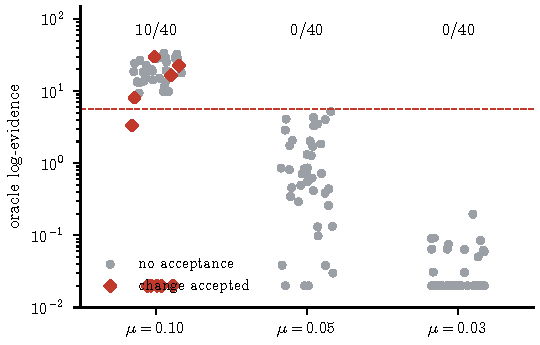
\includegraphics{figures/misadjustment.pdf}
\caption{Structureless targets with real inputs (development, 120 runs). Log-evidence of the best fixed-coefficient challenger (projection oracle) versus the acceptance threshold (dashed); red diamonds: runs where the model actually accepted a change (for those, the oracle was measured after the acceptance and can sit at the floor); numbers: accepted runs. The median oracle crosses the threshold at $\mu=0.1$ (\misOrcMedA) and stays below it at $\mu=0.05$ (maximum \misOrcMaxB).}
\label{fig:misadj}
\end{figure}

\paragraph{Verification.} With the reference learned by NLMS at $\mu=0.1$, \misAccA{} of 40 structureless targets had a change accepted. It was always the unit with the largest projection of $\eta$, the target's own past. At $\mu=0.05$ and $\mu=0.03$ there were \misAccB{} and \misAccC{} of 40 (\cref{fig:misadj}). LEBRE uses $\mu=0.05$, which is in the practical regime, \emph{not} in the exact one. False-change control is therefore checked empirically (\cref{sec:fdr}).

\section{Experimental protocol}\label{sec:protocol}

\paragraph{Task and metric.} Online one-step-ahead forecasting with the current inputs available; all models receive the same causally standardised inputs. The metric is the mean squared error on the last 70\% of each series (observed target), divided by that of an online NLinear calibrated on the same series, with the geometric mean across series. 95\% CIs come from a bootstrap stratified by domain (2{,}000 resamples, fixed seed). A series is \emph{catastrophic} when the relative error exceeds 10, the forecast deviates by more than 10 times the observed range, or the forecast is non-finite.

\paragraph{Data.} Hourly and daily hydro data from the Brazilian grid operator (ONS; cascaded plants, inputs = upstream flows), catchments of CAMELS-BR \citep{chagas2020camels} (inputs: precipitation, evapotranspiration, temperature), and heating and cooling meters of the Building Data Genome 2 \citep{miller2020bdg2} (inputs: weather). Series were split by seeded permutations, before any modelling, into development and reserves, and the loader refuses reserve series outside a pre-registered run. Development also used two system-identification benchmarks and declared synthetic suites.

\paragraph{Pre-registration.} Before each reserve was accessed, a document fixed the questions, metrics, comparators, criteria and code hashes. Each reserve was run once. Reserve 1 had 125 series (ONS 45, CAMELS-BR 50, BDG2 30), reserve 2 had 40 (CAMELS-BR 20, BDG2 20) and reserve 3 had 60 (CAMELS-BR 30, BDG2 30); the ONS rivers were exhausted after reserve 1.

\paragraph{Comparators.} The \emph{budget class} (up to $\sim10^4$ operations per forecast) contains:
\begin{itemize}
  \item online NLinear and DLinear \citep{zeng2023dlinear};
  \item online Holt--Winters;
  \item a dense ARX learned by NLMS and an online LASSO;
  \item FITS \citep{xu2024fits} and SparseTSF \citep{lin2024sparsetsf}, fitted on the first 15\% and then frozen;
  \item the previous LEBRE version (v0.51) as an ablation.
\end{itemize}
\emph{References} (ceilings, not opponents) are a SARIMAX with inputs fitted per series by maximum likelihood, a least-squares ARX with online order selection, TTM zero-shot and fine-tuned with the inputs as exogenous channels \citep{ekambaram2024ttm}, and Chronos-2 with covariates \citep{ansari2025chronos2}. Foundation models are too expensive to run at every step. They were therefore evaluated on 1{,}000 points per series, the same points for all models, with the current inputs given as known future covariates.

\paragraph{Microcontroller.} The canonical configuration was ported to C99 (float64 and float32) and compiled for a Cortex-M4F with \texttt{arm-none-eabi-gcc} 15.2 (\texttt{-O2}, single-precision FPU, no FMA contraction). It was run in Renode 1.17 \citep{renode} on an STM32F4 model, with the DWT cycle counter configured to count executed instructions. Cycles were estimated from execution traces with the published Cortex-M4 timings (zero-wait flash assumed). No physical board was used and energy was not measured.

\section{Results}\label{sec:results}

\subsection{Reserve 1: an engineering failure}\label{sec:res1}
The version evaluated in reserve 1 had no output safeguards, and 6 of 125 series exploded (relative error up to $10^{79}$). During long target gaps the memory filled its own history with its own forecasts, a recursion that some learned weights made unstable. The pre-registered result was dominated by these series (geometric mean \rOneAll). In an exploratory, non-pre-registered view without them, the relative error was 0.706. The safeguards of \cref{sec:method} were designed after seeing this failure, verified by a development stress test, and then evaluated on two new reserves. The fix was therefore not designed blind.

\subsection{Reserves 2 and 3}
\begin{figure}[t]
\centering
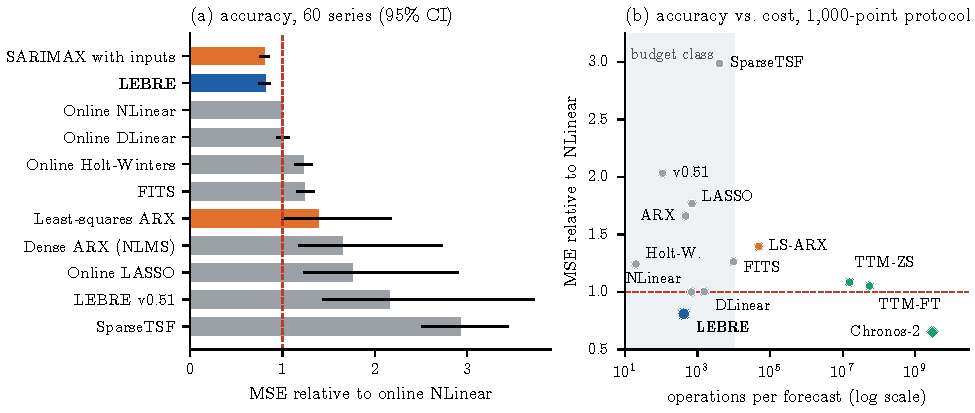
\includegraphics{figures/reserve3.pdf}
\caption{Reserve 3 (60 never-seen series). (a) MSE relative to online NLinear on the full test region, geometric mean with 95\% CIs (blue: LEBRE; grey: budget class; orange: classical references). (b) Error on the 1{,}000-point protocol versus operations per forecast (green: foundation models); the shaded band is the budget class. SARIMAX is omitted on the right because its per-forecast cost was not counted. The Chronos-2 cost (diamond) is an order-of-magnitude estimate.}
\label{fig:res3}
\end{figure}

\begin{table}[t]
\centering\small
\caption{Reserve 3, full test region (60 series). Relative MSE (geometric mean; lower is better), share of series with relative error above 1.5, catastrophic series and analytic operations per forecast.}
\label{tab:res3}
% generated by build_assets.py -- do not edit
\begin{tabular}{llrrlrrr}
\toprule
Model & Class & CAMELS & BDG2 & All [95\% CI] & $>1.5$ & Cat. & Ops/forecast\\
\midrule
\textbf{LEBRE} & budget & 0.858 & 0.768 & 0.812 [0.752, 0.866] & 0\% & 0 & 415 \\
SARIMAX with inputs & reference & 0.817 & 0.803 & 0.810 [0.763, 0.851] & 0\% & 0 & ML fit \\
Online NLinear & budget & 1.000 & 1.000 & 1.000 [1.000, 1.000] & 0\% & 0 & 674 \\
Online DLinear & budget & 1.076 & 0.947 & 1.009 [0.948, 1.066] & 3\% & 0 & 1,533 \\
Online Holt-Winters & budget & 1.213 & 1.244 & 1.229 [1.136, 1.323] & 25\% & 0 & 20 \\
FITS & budget & 1.362 & 1.137 & 1.244 [1.158, 1.335] & 18\% & 0 & 9,757 \\
Least-squares ARX & reference & 0.677 & 2.867 & 1.394 [0.998, 2.170] & 20\% & 4 & 48,944 \\
Dense ARX (NLMS) & budget & 1.008 & 2.711 & 1.653 [1.184, 2.730] & 38\% & 2 & 474 \\
Online LASSO & budget & 1.015 & 3.048 & 1.759 [1.237, 2.898] & 38\% & 4 & 705 \\
LEBRE v0.51 & budget & 2.180 & 2.140 & 2.160 [1.440, 3.723] & 48\% & 4 & 108 \\
SparseTSF & budget & 2.980 & 2.886 & 2.933 [2.512, 3.446] & 87\% & 3 & 4,016 \\
\bottomrule
\end{tabular}

\end{table}

\begin{table}[t]
\centering\small
\caption{Reserve 3, 1{,}000-point protocol with foundation models. Paired ratio LEBRE/model (geometric mean over series, 95\% CI); below 1 means LEBRE errs less.}
\label{tab:fm}
% generated by build_assets.py -- do not edit
\begin{tabular}{lrrrlrr}
\toprule
Model & CAMELS & BDG2 & All & Paired ratio & LEBRE wins & Ops/forecast\\
\midrule
\textbf{LEBRE} & 0.836 & 0.787 & 0.811 & -- & -- & $\approx$415 \\
SARIMAX with inputs & 0.798 & 0.818 & 0.808 & 1.004 [0.956, 1.056] & 28/60 & ML fit \\
TTM zero-shot & 1.204 & 0.978 & 1.085 & 0.747 [0.704, 0.795] & 57/60 & 15.6M \\
TTM fine-tuned (inputs) & 1.049 & 1.054 & 1.052 & 0.771 [0.699, 0.844] & 50/60 & 55.6M \\
Chronos-2 (covariates) & 0.782 & 0.539 & 0.649 & 1.250 [1.178, 1.337] & 9/60 & $\sim$1e9--1e10 \\
\bottomrule
\end{tabular}

\end{table}

\Cref{tab:res3,tab:fm} and \cref{fig:res3} report the pre-registered results of reserve 3; reserve 2 was consistent. The findings are:
\begin{itemize}
  \item \textbf{Budget class.} LEBRE had the lowest error among the budget-class comparators: \rThreeAll{} [\rThreeLo, \rThreeHi] on reserve 3 and \rTwoAll{} [\rTwoLo, \rTwoHi] on reserve 2. It had no catastrophic series and none above 1.5 in either reserve. Paired ratios against online DLinear and FITS were \pairDl{} and \pairFits.
  \item \textbf{Ultralight models in this regime.} FITS and SparseTSF, used here outside their design regime (one-step, frozen after fitting on 15\%), were behind online NLinear.
  \item \textbf{Classical reference.} LEBRE tied a SARIMAX with inputs fitted per series. The paired ratio was \pairSar{} [\pairSarLo, \pairSarHi] on reserve 3 and \rTwoSar{} on reserve 2.
  \item \textbf{Foundation models.} LEBRE's error was lower than TTM's, with ratios \pairTtmZ{} (zero-shot) and \pairTtmF{} (fine-tuned); these depend on the fine-tuning setup we chose in development. It was higher than that of Chronos-2 with covariates, with ratios \pairChr{} [\pairChrLo, \pairChrHi] on reserve 3 and \rTwoChr{} on reserve 2. The largest gap was on buildings (\kLebBdg{} vs.\ \kChrBdg).
  \item \textbf{Interval.} The 90\% interval had empirical coverage \covThree.
  \item \textbf{Cost.} The analytic cost averaged \fpMean{} operations per step, with a maximum of \fpMax. The contract declared beforehand was therefore \textbf{not met}, exceeded by \fpOverMean\% in the mean and \fpOverMax\% in the peak.
\end{itemize}

\subsection{C99 port and simulated microcontroller}
The float64 C build reproduced the Python decision sequences on \eqDevD/29 development series. The float32 build reproduced them on \eqDevF/29 development and \eqThree/60 reserve-3 series; in the others a decision near the threshold shifted by a few steps. On the simulated Cortex-M4F, the mean cost was \instrMin--\instrMax{} thousand instructions per step (\cref{tab:mcu,fig:mcu}). Peaks of \peakMin--\peakMax{} thousand instructions occurred only at decision steps. The estimated CPI was \cpiA{} and \cpiB, giving about \usMin--\usMax~$\mu$s per step at 168~MHz. The model state takes \stateKB~KB, dominated by a fixed-capacity hypothesis table: this fits an STM32F407 but not smaller microcontrollers without reducing capacities.

\begin{table}[t]
\centering\small
\caption{Simulated Cortex-M4F (float32 port): instructions per step, estimated time at 168~MHz (CPI 1.6), test-region NMSE (identical to Python) and accepted changes. Rows 4--7 belong to the pre-registered reserve 3.}
\label{tab:mcu}
% generated by build_assets.py -- do not edit
\begin{tabular}{lrrrrrrrr}
\toprule
Series & Inputs & Mean & Median & p99.9 & Peak & $\mu$s & NMSE & Changes\\
\midrule
ONS (dev.) & 1 & 3,703 & 3,363 & 12,327 & 42,021 & 35 & 0.2826 & 4 \\
CAMELS (dev.) & 3 & 4,560 & 4,599 & 14,387 & 48,447 & 43 & 0.0229 & 3 \\
BDG2 (dev.) & 2 & 5,964 & 5,607 & 16,843 & 45,654 & 57 & 0.0305 & 2 \\
CAMELS 51795000 & 3 & 3,203 & 3,003 & 12,223 & 36,771 & 31 & 0.1465 & 0 \\
CAMELS 64625000 & 3 & 3,521 & 3,215 & 12,267 & 36,708 & 34 & 0.3249 & 0 \\
BDG2 Fox\_education\_Ollie & 2 & 5,806 & 5,587 & 15,375 & 45,402 & 55 & 0.0162 & 3 \\
BDG2 Panther\_education\_Vincent & 2 & 5,528 & 5,463 & 16,971 & 45,696 & 53 & 0.0584 & 3 \\
\bottomrule
\end{tabular}

\end{table}

\begin{figure}[t]
\centering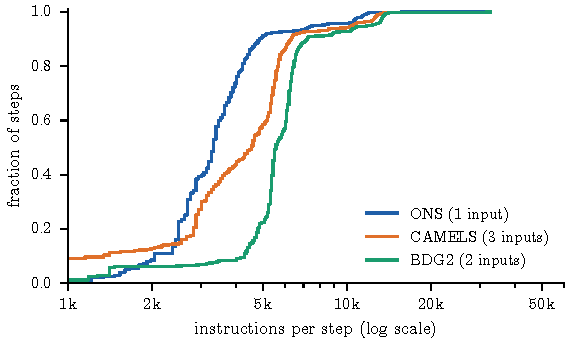
\includegraphics{figures/mcu_cdf.pdf}
\caption{Cumulative distribution of instructions per step on three development series (simulated Cortex-M4F). The cheapest steps have a missing target.}
\label{fig:mcu}
\end{figure}

\subsection{False-change control under dependence (simulation)}\label{sec:fdr}
We ran the frozen model on \simRuns{} synthetic runs of 30{,}000 steps (plan and criterion declared beforehand). The runs used four correlated inputs with persistence 0.5 or 0.95, four null scenarios and three scenarios with one true input. The nulls were white noise, an autoregressive target, noise whose variance depends on an input, and a variance break. The scenarios with a true input were plain, with a decoy correlated 0.7 with the true input, and with heavy-tailed autoregressive noise.
\begin{itemize}
  \item \textbf{Null scenarios.} \simNullFalse{} of \simNullRuns{} runs accepted any change.
  \item \textbf{Scenarios with a true input.} By the declared per-scenario criterion, all stayed within $\alpha=0.05$. With persistence 0.5, however, two cells exceeded it: FDR \simPTwoFdr{} (decoy, \simPTwoRuns/50 runs) and \simPThreeFdr{} (dependent noise, \simPThreeRuns/50) (\cref{fig:fdr}).
\end{itemize}
In all \simAffected{} affected runs, the false change was an input \emph{correlated} with the true one and accepted before it. While the true input is absent, such a substitute does improve the reference forecast: the test answers its own question correctly, but the answer is not structural. The periodic removal test took the substitute out in \simRemoved{} of \simAffected{} cases; in \simFinal{} of \simRuns{} runs it stayed in the final model. An accepted input therefore means ``improved the forecast of the current model, with evidence'', not ``is the cause''.

\begin{figure}[t]
\centering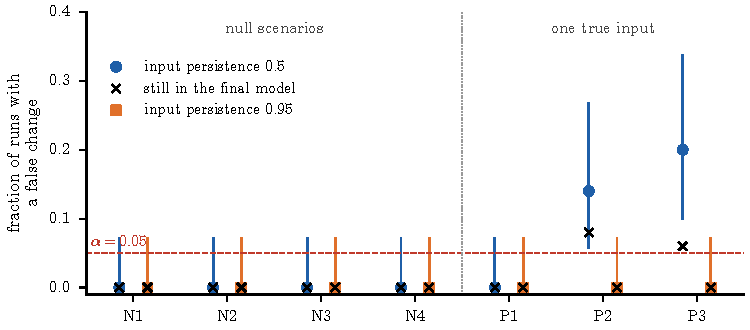
\includegraphics{figures/false_changes.pdf}
\caption{False-change simulation (700 runs; 50 per scenario and input persistence). Markers: fraction of runs with at least one false change, with Clopper--Pearson 95\% intervals; crosses: fraction where the false change was still in the final model.}
\label{fig:fdr}
\end{figure}

\subsection{Ablations}
\begin{itemize}
  \item \textbf{Testing mechanism.} Switching all units on from the start, without experiments, gave the same accuracy. On reserves 2 and 3 together (100 series, exploratory, because the reserves had already been used) the paired ratio LEBRE/all-on was \ablRatio{} [\ablLo, \ablHi], and the all-on version costs less (\ablCost{} vs.\ \fpMean{} operations per step). The testing mechanism is therefore not justified by accuracy: its role is an evidence-backed, logged structure, and its practical value for a downstream decision was \emph{not} demonstrated.
  \item \textbf{Output safeguards.} Without them, reserve 2 had \rTwoFrozenCat{} catastrophic series and a relative error of \rTwoFrozen{} (paired ratio \rTwoFrozenRatio{} in favour of the safeguards).
  \item \textbf{Other components.} Hierarchical splits made no difference on real data (ratio 0.996). Per-lag hypotheses (about 400 per series) instead of whole-input units were worse in development (0.757 vs.\ 0.645 on 1{,}000 points).
\end{itemize}

\section{Limitations}\label{sec:limits}
\begin{itemize}
  \item \textbf{Scope.} Two domains, 1--5 inputs, one step ahead with current inputs available; the last two reserves have no ONS series. With 40 and 60 series the confidence intervals are wide.
  \item \textbf{Statistics.} The e-values are valid under the stated assumptions, but with the adaptive reference false-change control is only empirical (\cref{sec:theory,sec:fdr}). Correlated substitutes can be accepted, near-identical inputs are indistinguishable, and very smooth inputs with medium or long delays are often not discovered. The last point is consistent with known power losses for persistent regressors \citep{stambaugh1999,campbell2006}. Removal tests rarely accept: with margin $-0.002$ the evidence for removing a useless unit grows slowly relative to the episode length.
  \item \textbf{Comparisons.} SARIMAX, FITS, SparseTSF and TTM were fitted once in batch; online ARMAX/Kalman variants were not evaluated. The fine-tuning of TTM used one configuration chosen in development. Foundation models were evaluated on 1{,}000 points per series.
  \item \textbf{Cost.} The declared contract was not met. The microcontroller results come from a simulator, cycles are estimated from traces, and energy was not measured.
  \item \textbf{Process.} The output safeguards were designed after the failure of reserve 1. The cost contract was revised once during development. The literature search behind \cref{sec:related} used one search engine and mostly abstracts.
\end{itemize}

\section{Discussion and conclusion}
At a mean cost of \fpMean{} operations per step and in the tested domains, a simple online linear model with a seasonal memory and output safeguards delivered competitive one-step forecasts without catastrophic failures. It tied a per-series SARIMAX and stayed within about 25\% of a large foundation model with covariates. The evidence-gated structural mechanism did not add accuracy. What it adds is an auditable record of which inputs and delays entered the model, when and with what evidence. We also make explicit a condition under which such a record may be read structurally: the reference that challengers are compared against must have small misadjustment. When correlated substitutes exist, even that reading is only about predictive relevance. Natural next steps are:
\begin{itemize}
  \item a reference with provably small misadjustment (a slow shadow reference);
  \item online ARMAX/Kalman comparators;
  \item a physical board with energy measurement;
  \item a smaller state;
  \item evaluation in further domains;
  \item a demonstration that the logged structure improves a downstream decision.
\end{itemize}

\section*{Reproducibility statement}
The frozen research implementation and the reproducibility record are available at \url{https://github.com/Iquitim/lebre-research} and archived as \href{https://doi.org/10.5281/zenodo.23049103}{doi:10.5281/zenodo.23049103}. The installable library implementing this frozen version is available at \url{https://github.com/Iquitim/lebre}. The record contains the Python reference implementation, the C99 port and firmware, all experiment scripts, the pre-registrations with their hashes, per-series result tables, reports and SHA-256 manifests of every frozen version. Every number in this paper is generated from result files by a script (\texttt{paper/build\_assets.py}). A smoke test re-runs the frozen model on reserve series and reproduces the published predictions bit for bit. Raw third-party data and per-series prediction arrays are not in the repository; they are listed with SHA-256 checksums. The library reproduces the reference predictions bit for bit in the reference environment and up to floating-point rounding elsewhere, with identical structural decisions in its regression tests.

\section*{Use of generative AI}
Generative AI tools (Anthropic's Claude) were used to assist with code, analysis scripts, figures and drafting of the text. The author reviewed all content and takes full responsibility for it.

\bibliographystyle{plainnat}
\bibliography{refs}

\clearpage
\appendix
\section{Constants}\label{sec:params}
\begin{table}[h]
\centering\small
\caption{Constants of the evaluated configuration (identical for all series).}\label{tab:params}
\begin{tabularx}{\linewidth}{lX}
\toprule
Group & Constants\\
\midrule
Units & one per input (incl.\ the target's own past) + residual latent state (poles 0.8, 0.95); at most 4 active\\
Response & bands [1], [2--3], [4--7], [8--15], [16--31] + peak lag (chosen after 200 samples) + current value; splits into halves\\
Challengers & RLS within episode, $P_0=10I$; warm-up 250; 2 slots; one warm-up at a time\\
Evidence & $\ell=\min\{e^2/B^2,1\}$, $B=2\max(\hat\sigma_S,0.1 s^{\mathrm{slow}})$; $c=1+\max(\varepsilon,0)$; 8 values $\lambda_j=0.9\cdot2^{-j}/c$; $\varepsilon=+0.002$ (add, swap, split), $-0.002$ (remove)\\
Multiplicity & $\alpha=0.05$; $\gamma=1/(2P)$ for the first $P=2\cdot\#$units, then $0.5\,\gamma_k\propto 1/(k\log^2k)$; level $\min(\alpha\gamma(R+1),0.5)$\\
Episodes & scan rule after 100 samples; cap 5{,}000; cool-down 2{,}000; removal test every 2{,}000; decisions every 10 steps\\
Screening & prewhitened AR(1), EMA weight 0.02, every 4 steps per part; thresholds 15.09 ($\chi^2_5$), 6.63 ($\chi^2_1$)\\
Base of $S$ & NLMS $\mu=0.05$; input contract $\pm8\sigma$ with 31-step quarantine\\
Memory & NLMS $\mu=0.05$; slow mean 0.01; profile 0.1; floors $10^{-3}$, $10^{-4}$; declared cycle(s); hold during gaps\\
Combination, output & $\lambda=0.99$, $\eta=0.5$, every 8 steps; envelope rate $10^{-3}$, margin $0.5\times$\\
Interval & target 90\%, gain 0.1, every 8 steps\\
Inputs & causal standardisation, exponential rate $10^{-4}$ from mean 0 / variance 1\\
\bottomrule
\end{tabularx}
\end{table}

\end{document}
